\section{Results \& Discussion}

In this section, the results from the implementation of the code for a specific example are shown. The image that was analysed as an example, as well as its imported and processed states, are shown in Figure \ref{fig:load&processing}.

\begin{figure}[h] %  figure placement: here, top, bottom, or page
    \centering
    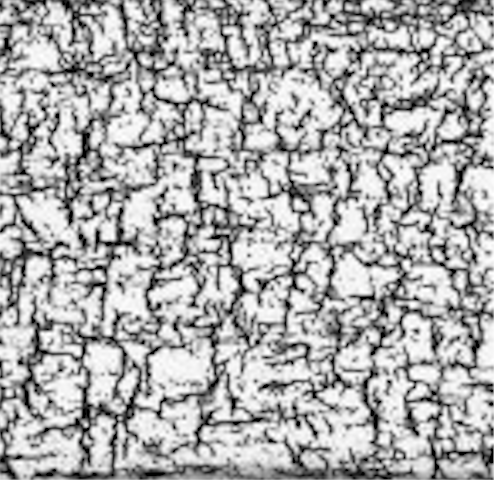
\includegraphics[width=1.8in]{Figures/5-Results/chu7.jpg}
    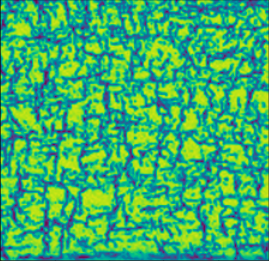
\includegraphics[width=1.8in]{Figures/5-Results/loading.PNG}
    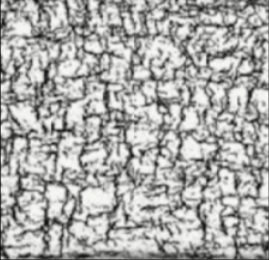
\includegraphics[width=1.8in]{Figures/5-Results/processing.PNG}
    \caption{Image to be analysed: a) Original state, b) After loading, c) After processing.}
    \label{fig:load&processing}
\end{figure}

\noindent
In Figure \ref{fig:thresholding}, it can be observed the image after the three different threshold were applied: Otsu, K-means and Gauss. The K-means threshold seems to be the most clear of them so far.

\begin{figure}[h] %  figure placement: here, top, bottom, or page
    \centering
    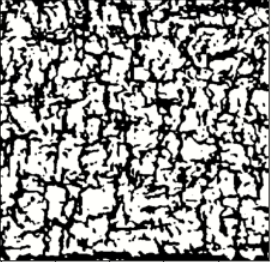
\includegraphics[width=1.8in]{Figures/5-Results/ThOtsu.PNG}
    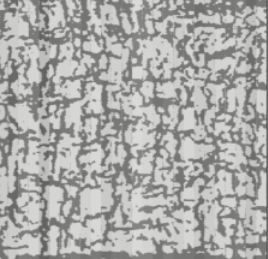
\includegraphics[width=1.8in]{Figures/5-Results/ThKmeans.PNG}
    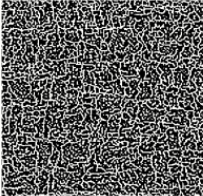
\includegraphics[width=1.8in]{Figures/5-Results/ThGauss.PNG}
    \caption{Images after three different thresholds were applied: a) Otsu b) K-means, c) Gauss.}
    \label{fig:thresholding}
\end{figure}

\noindent
In Figure \ref{fig:connectivity}, it can be observed the resulting images after studying the connectivity between hydrides in the radial direction. Due to the inconsistent quality of thresholding obtained by the Gaussian method, the image obtained from the Gauss thresholding was excluded from HCC analysis. The other two images were subjected to the HCC analysis. 

Two methods were followed to calculate the HCC value. With the first one, the HCC value is calculated for every single pixel column and all the numbers are averaged to give a resulting HCC value. This method was discarded because the results (0.11 for Otsu thresholding and 0.13 for K-means thresholding) were too low for their corresponding connectivity images (Fig. \ref{fig:connectivity} a and b, respectively). The images show a big amount of radial hydrides, so it is expectable to obtain a higher value of HCC.

With the second method, the HCC value of every slice is measured, and then the values are averaged. The results of the second method fit better their corresponding images. The HCC value for the image Otsu-thresholed is the same as for the K-means thresholded: 0.65. 

\begin{figure}[h] %  figure placement: here, top, bottom, or page
    \centering
    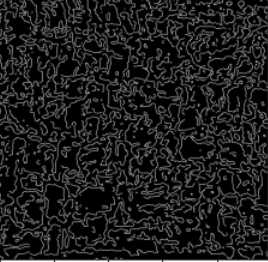
\includegraphics[width=1.8in]{Figures/5-Results/Otsu.PNG}
    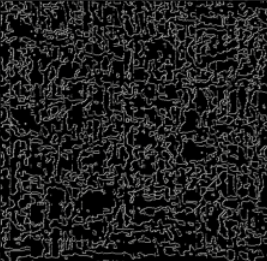
\includegraphics[width=1.8in]{Figures/5-Results/Kmeans.PNG}
    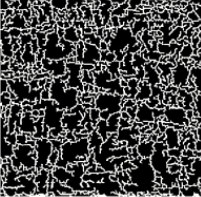
\includegraphics[width=1.8in]{Figures/5-Results/Gauss.PNG}
    \caption{Connectivity of the images with a) Otsu threshold, b) K-means threshold, c) Gauss threshold.}
    \label{fig:connectivity}
\end{figure}

This model was used in different images for comparison. The images analysed and their corresponding HCC values obtained after Otsu and K-means thresholdings are shown in Figure \ref{fig:compa}. As can be expected, the highest values of HCC are obtained for the microstructure showed in Fig 12a, which has many hydrides in both directions, longitudinal and radial, and therefore, the connectivity is favoured. When the majority of the hydrides are longitudinal, as in Fig 12b, the HCC value is lower. If we compare Fig12 a and c, the main difference between these microstructures is the amount of hydrides. The microstructure a has higher values of HCC than the microstructure c. Finally, the microstructure d shows less longitudinal hydrides than the microstructure b, so the HCC is also lower.


\begin{figure}[h] %  figure placement: here, top, bottom, or page
    \centering
    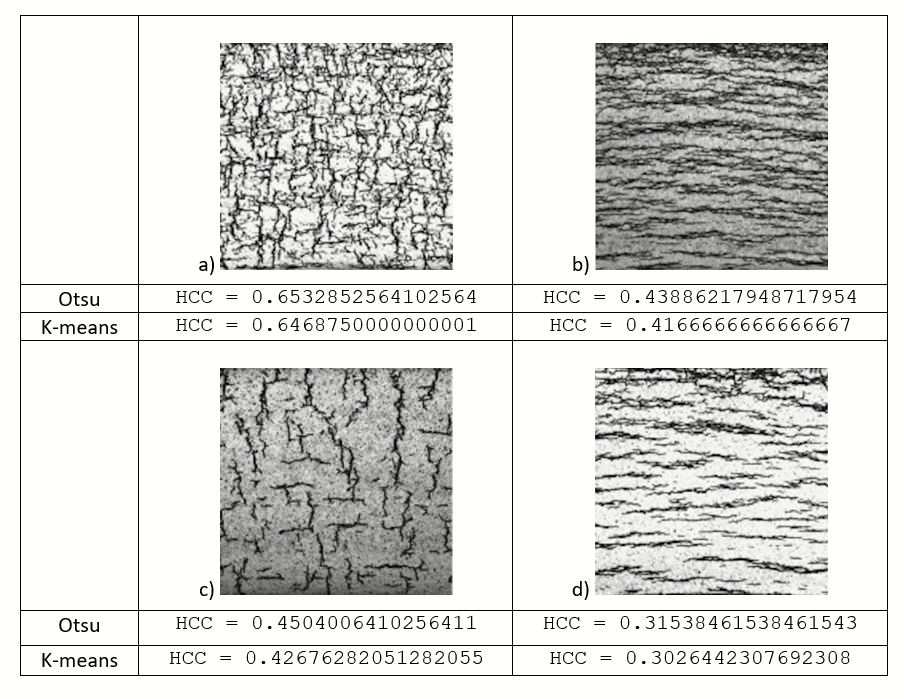
\includegraphics[width=5.5in]{Figures/5-Results/Comparison.PNG}
    \caption{HCC values for different microstructures: a) Many longitudinal and radial hydrides, b) Majority of longitudinal hydrides, c) Some longitudinal and radial hydrides, d) Some longitudinal hydrides.}
    \label{fig:compa}
\end{figure}